\documentclass[11pt]{article}
\usepackage[a4paper,margin=2.6cm]{geometry}
\usepackage[T1]{fontenc}
\usepackage[utf8]{inputenc}
\usepackage{lmodern}
\usepackage{amsmath,amssymb}
\usepackage{graphicx}
\usepackage{booktabs}
\usepackage{caption}
\usepackage[hidelinks]{hyperref}
\usepackage{microtype}
\graphicspath{{../figures/}}
\captionsetup{font=small,labelfont=bf}

\title{Classical versus Quantum Machine Learning for Credit Default
Prediction:\\ An Honest Benchmark at Matched Sample Sizes}
\author{Nicol\`o Angileri\\
\small Mediterranean Quantitative Finance Society (MQFS) --- Working Paper}
\date{}

\begin{document}
\maketitle

\begin{abstract}
\noindent We benchmark three classical credit-scoring models against two
quantum machine-learning models --- a fidelity quantum-kernel support vector
classifier (QK-SVC) and a variational quantum classifier (VQC) --- on the UCI
``Default of Credit Card Clients'' dataset (30{,}000 real Taiwanese
credit-card accounts). The evaluation is finance-aware: beyond AUC, PR-AUC and
calibration, we score every model under an asymmetric expected-loss matrix and
NT\$ profit curves over the approval threshold. Because fidelity kernels cost
$O(n^2)$ circuit evaluations, quantum models can only be trained on small
subsamples; our central methodological rule is that \emph{classical baselines
are re-trained on exactly the same subsamples} ($n \in \{500, 1000, 2000\}$, three
independent draws), so no comparison ever crosses sample sizes. At every
matched size the best classical model matches or exceeds both quantum models
(at $n=2000$: best classical test AUC 0.7691 vs.\ best quantum
0.7007, a gap of 0.0684), while training orders of magnitude faster.
\textbf{No quantum advantage is claimed --- or observed --- in this regime.}
The contribution is the protocol and the measured operating envelope: an
honest, reproducible baseline that future quantum-hardware claims on tabular
credit risk can be checked against. All numbers regenerate from one command in
about 7 minutes on a laptop.
\end{abstract}

\section{Introduction}
Credit scoring is one of the oldest industrial applications of statistical
learning \cite{hand1997,thomas2002}, and one of the most heavily benchmarked
\cite{lessmann2015}. It is also, lately, a popular showcase for quantum
machine learning (QML), where quantum feature maps promise classically
intractable kernels \cite{havlicek2019,schuld2019}. Provable quantum speedups
for supervised learning exist only for contrived problems
\cite{liu2021}; whether \emph{any} benefit survives contact with a real,
noisy, tabular credit dataset at the sample sizes quantum methods can actually
process is an empirical question --- and one that is easy to answer
misleadingly. A recurring failure mode in applied QML papers is the uneven
comparison: a quantum model trained on hundreds of points is compared against
a classical model trained on the full dataset (or vice versa), with accuracy
as the only metric and wall-clock cost unreported.

This working paper does the boring version of the experiment, deliberately.
Our contributions are methodological:
(i) a \emph{matched-subsample fairness rule} --- every classical baseline is
re-trained on the exact stratified subsamples the quantum models use;
(ii) a \emph{finance-aware evaluation} --- an asymmetric expected-loss matrix
with its Bayes-optimal operating threshold, and portfolio profit curves in
NT\$ using each client's actual credit limit as exposure;
(iii) \emph{honest cost accounting} --- wall-clock time for every phase of
every model, including quantum state preparation; and
(iv) full reproducibility --- fixed seeds, defensive data validation,
known-answer unit tests (kernel symmetry/PSD, cost-matrix algebra), and a
single command that regenerates every number and figure in this paper.

\section{Data}
We use the UCI ``Default of Credit Card Clients'' dataset (id 350)
\cite{yeh2009,uci}: 30{,}000 Taiwanese credit-card clients observed in
October 2005, 23 raw features (credit limit, demographics, six months of
repayment status \texttt{PAY\_0, PAY\_2--PAY\_6}, bill and payment amounts),
and a binary target --- default on the next monthly payment. The default rate
is 22.12\% (6,636 of 30,000); classes are imbalanced but not
extremely so. The raw \texttt{.xls} is fetched once and cached (SHA-256
recorded in \texttt{results/data\_manifest.json}); a defensive parser
validates the documented schema (exact row count, value ranges, no missing
values) before any modelling. Cleaning is minimal and fully documented in
\texttt{docs/DATA\_NOTES.md}: undocumented \texttt{EDUCATION} codes
$\{0,5,6\}$ (345 cells) and \texttt{MARRIAGE} code $0$ (54
cells) are collapsed into their ``others'' categories; no rows are dropped;
no values are imputed. We hold out a fixed stratified 25\% test set
($n_{\text{test}} = 7,500$, seed 42) used by \emph{every} model in this
paper; all tuning happens inside the training set.

\section{Methodology}
\subsection{Classical models and protocol}
Three standard baselines are trained on the full training set
($n = 22,500$): $\ell_2$ logistic regression with balanced class weights
and isotonic probability calibration; a random forest (400 trees, balanced
subsample weights); and histogram gradient boosting (HGB) with balanced class
weights. Categorical variables are one-hot encoded and numerics standardised
for the linear model inside the pipeline (no leakage); tree ensembles consume
the raw integer-coded features. We report 5-fold stratified cross-validation
means $\pm$ standard deviations, held-out test metrics, and quantile-binned
reliability diagrams. Operating thresholds are selected on out-of-fold
training predictions only, then applied unchanged to the test set.

\subsection{Finance-aware, cost-sensitive evaluation}
Accuracy is the wrong loss for lending. Let $y_i = 1$ denote default and let
a model reject applicant $i$ when its predicted default probability $p_i$
exceeds a threshold $t$. With unit costs $c_{\mathrm{FN}}$ (approving a
future defaulter) and $c_{\mathrm{FP}}$ (rejecting a good client), the
empirical expected cost per applicant is
\begin{equation}
\widehat{C}(t) \;=\; \frac{1}{n}\Big( c_{\mathrm{FN}} \,\mathrm{FN}(t)
 \;+\; c_{\mathrm{FP}} \,\mathrm{FP}(t) \Big),
\label{eq:cost}
\end{equation}
and for perfectly calibrated probabilities the Bayes-optimal rule rejects iff
$p \ge t^\ast$ with
\begin{equation}
t^\ast \;=\; \frac{c_{\mathrm{FP}}}{c_{\mathrm{FP}} + c_{\mathrm{FN}}}
\label{eq:bayes}
\end{equation}
\cite{elkan2001}. We adopt the classic credit-scoring asymmetry
$c_{\mathrm{FN}} : c_{\mathrm{FP}} = 5 : 1$, giving $t^\ast = 1/6 \approx
0.167$; the distance between a model's empirical cost-minimising threshold
and $t^\ast$ is itself a calibration diagnostic. Complementarily, we compute
portfolio profit with heterogeneous exposures, approving iff $p_i < t$:
\begin{equation}
\Pi(t) \;=\; \sum_{i\,:\,p_i < t} \Big[ (1-y_i)\, m\, L_i \;-\; y_i\,
\lambda\, L_i \Big],
\label{eq:profit}
\end{equation}
where $L_i$ is client $i$'s actual credit limit (\texttt{LIMIT\_BAL}, in
NT\$), $m = 0.10$ a stylised revenue margin on performing accounts and
$\lambda = 0.60$ a stylised loss-given-default fraction. These economic
parameters are illustrative and clearly flagged as such; the full curves over
$t$ (Figure~\ref{fig:costprofit}) expose the sensitivity.

\subsection{Fidelity quantum kernel}
Following Havl\'i\v{c}ek et al.\ \cite{havlicek2019}, data are embedded by
the second-order Pauli-Z feature map $\mathcal{U}_{\Phi(x)}$
(\texttt{ZZFeatureMap}, 2 repetitions): after Hadamards, single- and
two-qubit phase rotations with angles $\phi_i(x) = x_i$ and $\phi_{ij}(x) =
(\pi - x_i)(\pi - x_j)$. The kernel is the state fidelity
\begin{equation}
K(x, x') \;=\; \bigl|\langle \Phi(x) \,|\, \Phi(x') \rangle\bigr|^2,
\label{eq:kernel}
\end{equation}
consumed by a standard SVC with balanced class weights (precomputed Gram
matrix; $C$ chosen by inner 3-fold CV over the same grid as the classical
RBF-SVC, its exact classical twin). On real hardware $K$ is estimated by the
compute--uncompute circuit
$\mathcal{U}_{\Phi(x')}^{\dagger}\mathcal{U}_{\Phi(x)}|0\rangle^{\otimes d}$
(probability of the all-zeros outcome); on the statevector simulator used
here Eq.~\eqref{eq:kernel} is evaluated exactly, i.e.\ our quantum results
are \emph{noise-free upper bounds} on NISQ performance. Since features must
fit $d$ qubits, we select the top-$d$ features by mutual information with the
label ($d = 4$ primary, $d = 8$ robustness), estimated on each training
subsample only, then min--max scale them to angles in $[0, \pi]$ (test values
clipped to the training range). MI selection is preferred over PCA to keep
the encoded features interpretable and to avoid rotating integer-coded
categoricals into dense components; PCA is implemented as an alternative.

\subsection{Variational quantum classifier}
The VQC applies a RealAmplitudes ansatz $U(\theta)$ (3 entangling
repetitions, 16 parameters at $d = 4$) to the same feature-map
states and measures the qubit-parity observable
$P = Z^{\otimes d}$:
\begin{equation}
p(x;\theta) \;=\; \tfrac{1}{2}\Bigl(1 - \langle\Phi(x)| U(\theta)^{\dagger} P\,
U(\theta) |\Phi(x)\rangle\Bigr),
\label{eq:vqc}
\end{equation}
trained by COBYLA (250 iterations, 2 restarts, best
kept) on class-weighted cross-entropy. Because $P$ is diagonal and the
feature-map states are cached, each objective evaluation reduces to applying
one $2^d \times 2^d$ unitary to the cached state matrix --- exact simulation,
reported timings included.

\subsection{The fairness rule}
Building the Gram matrix costs $O(n^2)$ kernel evaluations ($\sim$2M circuits
at $n = 2000$ on hardware), so quantum models are trained on stratified
subsamples $n \in \{500, 1000, 2000\}$ with three independent draws (seeds 0/1/2).
\textbf{Every classical baseline is re-trained on exactly the same
subsamples.} All models --- classical and quantum, every size --- are
evaluated on the same fixed 7,500-client test set, and decision costs are
compared at the same fixed Bayes threshold $t^\ast = 1/6$ (no per-model
threshold tuning at small $n$). We never compare quantum-on-2000 with
classical-on-22,500.

\section{Results}
\subsection{Part 1 --- classical baselines on the full training set}
Table~\ref{tab:full} summarises the full-data study.
Gradient boosting (HGB) performs best (test AUC 0.7774, PR-AUC 0.5528,
Brier 0.1792). Reliability diagrams (Figure~\ref{fig:calib}) show
the isotonic-calibrated logistic model closest to the diagonal, consistent
with its empirical cost-optimal threshold landing nearest the Bayes value
$t^\ast = 1/6$ (Eq.~\ref{eq:bayes}): Logistic regression (calibrated) $\hat t = 0.162$; Random forest $\hat t = 0.282$; Gradient boosting (HGB) $\hat t = 0.404$. Cost and profit curves are
shown in Figure~\ref{fig:costprofit}; at its out-of-fold profit-optimal
threshold, Gradient boosting (HGB) attains NT\$34.2M on the test portfolio
at an approval rate of 45.3\%.

\begin{table}[t]
\centering\small
\caption{Full-training-set classical baselines ($n=22,500$; test
$n=7,500$). CV: 5-fold stratified mean $\pm$ std. Cost per applicant
(Eq.~\ref{eq:cost}) at the OOF-selected threshold; profit (Eq.~\ref{eq:profit})
in NT\$ millions.}
\label{tab:full}
\begin{tabular}{lccccccc}
\toprule
Model & CV AUC & Test AUC & PR-AUC & Brier & Cost@$t^\ast_{\text{OOF}}$ &
Profit (M) & Fit (s) \\
\midrule
Logistic regression (calibrated) & 0.7281 $\pm$ 0.0072 & 0.7189 & 0.4966 & 0.1424 & 0.6376 & 17.6 & 1.9 \\
Random forest & 0.7795 $\pm$ 0.0046 & 0.7721 & 0.5527 & 0.1495 & 0.5736 & 30.8 & 3.7 \\
Gradient boosting (HGB) & 0.7822 $\pm$ 0.0059 & 0.7774 & 0.5528 & 0.1792 & 0.5612 & 34.2 & 0.1 \\
\bottomrule
\end{tabular}
\end{table}

\paragraph{What drives default risk.} Permutation importance on the test set
(Figure~\ref{fig:imp}) is dominated by the most recent repayment status
\texttt{PAY\_0}, followed by \texttt{LIMIT\_BAL}, \texttt{BILL\_AMT1} --- recent delinquency, not
demographics, carries the signal, in line with the credit-scoring literature
\cite{yeh2009,lessmann2015}. Top-5 AUC drops: \texttt{PAY\_0} (0.083), \texttt{LIMIT\_BAL} (0.018), \texttt{BILL\_AMT1} (0.016), \texttt{PAY\_AMT3} (0.010), \texttt{PAY\_AMT1} (0.007).

\subsection{Part 2 --- matched subsamples: the honest comparison}
Table~\ref{tab:matched} is the central result. At every matched training size
the best classical model is at least as good as the best quantum model; at
$n = 2000$ the gap between the best classical (Random forest,
0.7691) and the best quantum (QK-SVC, fidelity kernel, $d$=8, 0.7007) is
0.0684 AUC. The quantum kernel at $d=8$ trails $d=4$ at the two smaller
sizes and edges past it only at $n=2000$, remaining well below every
classical baseline; the VQC trails throughout, as expected for a
16-parameter model. In expected-cost terms (Table~\ref{tab:cost})
the classical RBF-SVC is the cheapest decision-maker at every size; the
Platt-calibrated quantum-kernel probabilities are competitive with the tree
ensembles at this fixed threshold --- a calibration effect, not a ranking
reversal. The VQC's parity-derived probabilities concentrate near $0.5$, so
at the fixed $1/6$ threshold it rejects essentially the whole portfolio: its
expected cost sits at the reject-all bound. Figure~\ref{fig:aucn} overlays learning
curves; Figure~\ref{fig:timing} shows honest wall-clock costs --- the QK-SVC
pays a large simulation overhead (dominated by test-set embedding and the
$n_{\text{test}} \times n$ kernel block), and on hardware the same object
would cost millions of shots. Figure~\ref{fig:gram} visualises a Gram
sub-block: within-class and between-class fidelities are barely
distinguishable, a first hint of why the kernel does not separate this data
better than its classical twin.

\begin{table}[t]
\centering\small
\caption{Matched-subsample test AUC (mean $\pm$ std over 3 identical
stratified draws; C = classical, Q = quantum). Same subsamples, same test
set, same threshold rule for every model.}
\label{tab:matched}
\begin{tabular}{lcccc}
\toprule
Model & $n=500$ & $n=1000$ & $n=2000$ & Time@2000 (s) \\
\midrule
Logistic regression (calibrated) (C) & 0.6949 $\pm$ 0.0267 & 0.7118 $\pm$ 0.0033 & 0.7148 $\pm$ 0.0017 & 0.0 \\
Random forest (C) & 0.7513 $\pm$ 0.0060 & 0.7613 $\pm$ 0.0013 & 0.7691 $\pm$ 0.0042 & 0.6 \\
Gradient boosting (HGB) (C) & 0.7038 $\pm$ 0.0085 & 0.7158 $\pm$ 0.0093 & 0.7352 $\pm$ 0.0114 & 0.3 \\
SVC, RBF kernel (classical twin) (C) & 0.7193 $\pm$ 0.0070 & 0.7368 $\pm$ 0.0038 & 0.7486 $\pm$ 0.0051 & 1.5 \\
QK-SVC, fidelity kernel, $d$=4 (Q) & 0.6875 $\pm$ 0.0026 & 0.7011 $\pm$ 0.0119 & 0.6891 $\pm$ 0.0247 & 7.2 \\
QK-SVC, fidelity kernel, $d$=8 (Q) & 0.6643 $\pm$ 0.0173 & 0.6812 $\pm$ 0.0137 & 0.7007 $\pm$ 0.0029 & 28.4 \\
VQC, $d$=4 (Q) & 0.6936 $\pm$ 0.0040 & 0.6811 $\pm$ 0.0189 & 0.6713 $\pm$ 0.0210 & 7.1 \\
\bottomrule
\end{tabular}
\end{table}

\begin{table}[t]
\centering\small
\caption{Expected cost per applicant (Eq.~\ref{eq:cost}) at the fixed Bayes
threshold $t^\ast = 1/6$; lower is better.}
\label{tab:cost}
\begin{tabular}{lccc}
\toprule
Model & $n=500$ & $n=1000$ & $n=2000$ \\
\midrule
Logistic regression (calibrated) & 0.6862 $\pm$ 0.0286 & 0.6960 $\pm$ 0.0102 & 0.6871 $\pm$ 0.0100 \\
Random forest & 0.6685 $\pm$ 0.0115 & 0.6516 $\pm$ 0.0090 & 0.6389 $\pm$ 0.0204 \\
Gradient boosting (HGB) & 0.7300 $\pm$ 0.0254 & 0.6948 $\pm$ 0.0120 & 0.6386 $\pm$ 0.0176 \\
SVC, RBF kernel (classical twin) & 0.6402 $\pm$ 0.0117 & 0.6251 $\pm$ 0.0107 & 0.6007 $\pm$ 0.0151 \\
QK-SVC, fidelity kernel, $d$=4 & 0.6670 $\pm$ 0.0193 & 0.6321 $\pm$ 0.0081 & 0.6288 $\pm$ 0.0150 \\
QK-SVC, fidelity kernel, $d$=8 & 0.7060 $\pm$ 0.0327 & 0.6732 $\pm$ 0.0067 & 0.6574 $\pm$ 0.0062 \\
VQC, $d$=4 & 0.7788 $\pm$ 0.0000 & 0.7787 $\pm$ 0.0001 & 0.7796 $\pm$ 0.0015 \\
\bottomrule
\end{tabular}
\end{table}

\subsection{Hardware estimation path}
The repository implements this estimator behind an explicit \texttt{--hardware} flag (\texttt{experiments/run\_hardware.py}): it reads the user's saved \texttt{QiskitRuntimeService} account from \verb|~/.qiskit| (tokens never enter the repository), submits one job of at most 28 compute--uncompute circuits to the least-busy backend, and reports measured versus simulated kernel entries. It was \emph{not} executed for this draft: the build environment holds no QPU credentials, and the tables above are exact-simulation results by design. Hardware numbers, when produced, land in \texttt{results/hardware\_kernel.json} and are reported verbatim.

\begin{figure}[t]
\centering
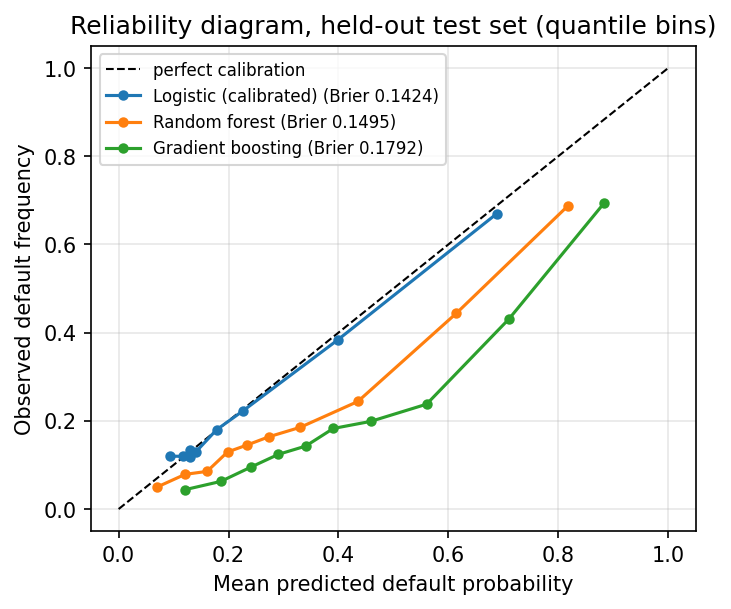
\includegraphics[width=0.62\textwidth]{calibration_full.png}
\caption{Reliability diagrams on the held-out test set (quantile bins).}
\label{fig:calib}
\end{figure}

\begin{figure}[t]
\centering
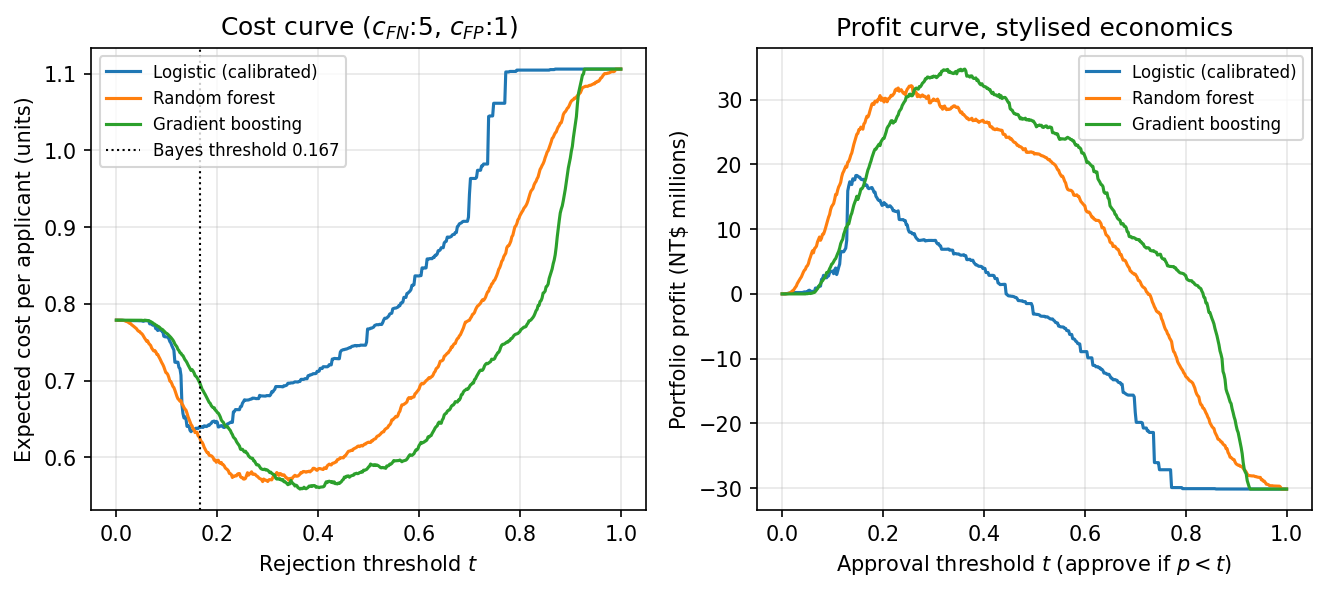
\includegraphics[width=0.95\textwidth]{cost_profit_full.png}
\caption{Left: expected cost per applicant vs.\ rejection threshold, with the
Bayes threshold $t^\ast = 1/6$. Right: NT\$ portfolio profit vs.\ approval
threshold under the stylised economics of Eq.~\eqref{eq:profit}.}
\label{fig:costprofit}
\end{figure}

\begin{figure}[t]
\centering
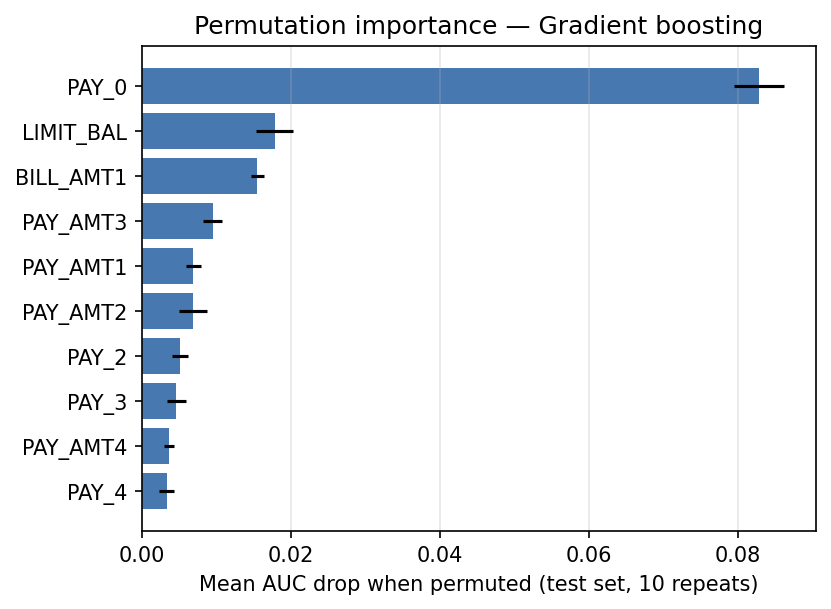
\includegraphics[width=0.7\textwidth]{permutation_importance.png}
\caption{Permutation feature importance (test set, 10 repeats) for the best
full-data model.}
\label{fig:imp}
\end{figure}

\begin{figure}[t]
\centering
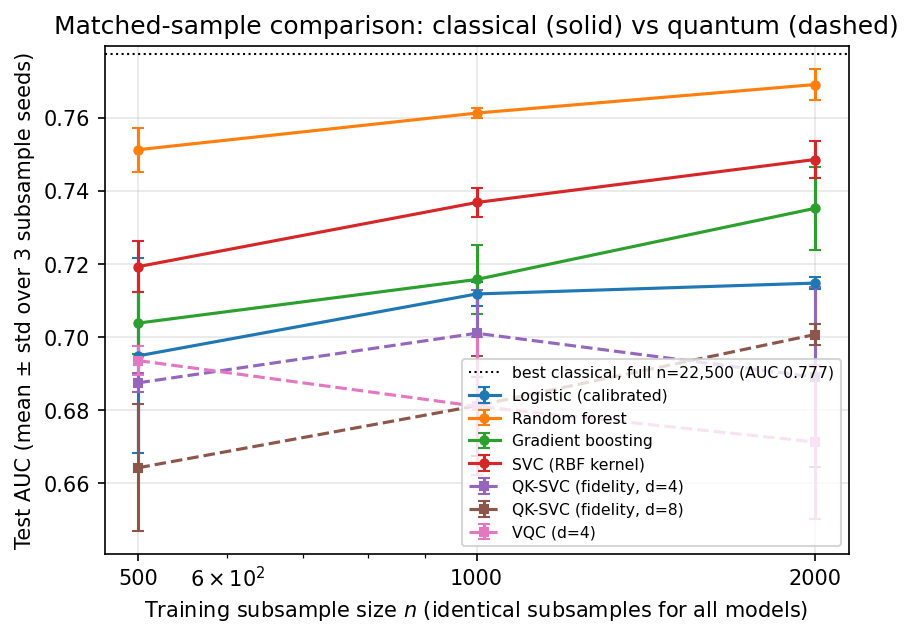
\includegraphics[width=0.72\textwidth]{auc_vs_n.png}
\caption{Matched-sample learning curves: classical (solid) vs.\ quantum
(dashed), mean $\pm$ std over three identical subsample draws.}
\label{fig:aucn}
\end{figure}

\begin{figure}[t]
\centering
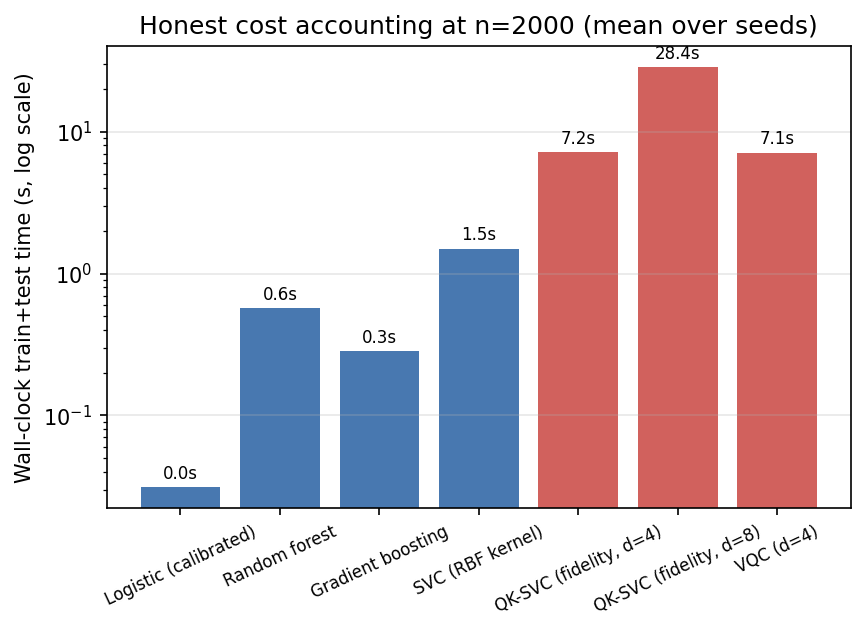
\includegraphics[width=0.62\textwidth]{timing.png}
\caption{Honest wall-clock accounting at $n=2000$ (log scale). Quantum
timings are exact-statevector simulation; hardware execution would add shot
and queue overheads.}
\label{fig:timing}
\end{figure}

\begin{figure}[t]
\centering
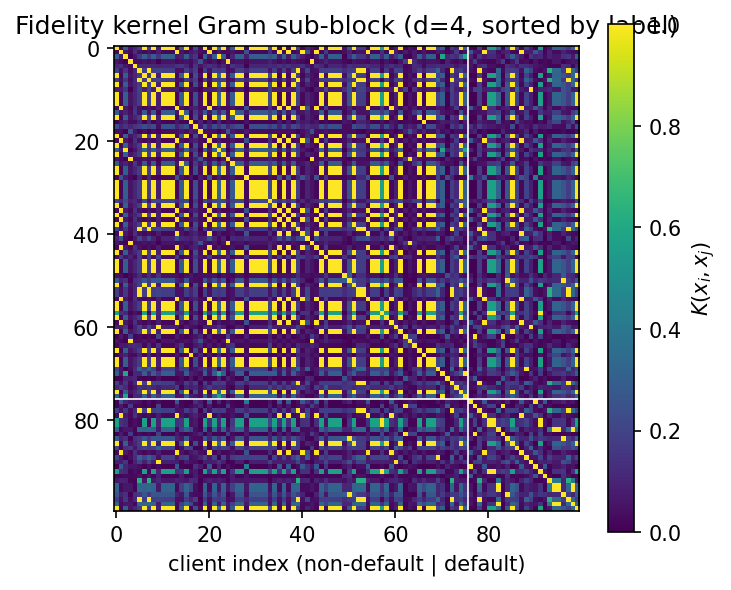
\includegraphics[width=0.55\textwidth]{kernel_gram.png}
\caption{Fidelity-kernel Gram sub-block ($d=4$, 100 training points sorted
by label).}
\label{fig:gram}
\end{figure}

\section{Limitations}
This is a single dataset, from 2005, from one market; conclusions are about
the \emph{measured regime}, not about QML in general. The economic parameters
$(c_{\mathrm{FN}}\!:\!c_{\mathrm{FP}}, m, \lambda)$ are stylised; profit
levels shift with them even though model rankings here do not. Quantum models
were simulated exactly (no shot noise, no device noise): real-hardware
results would be strictly worse, which only strengthens the negative finding,
but we did not measure the degradation beyond providing the estimator.
Feature compression to $d \in \{4, 8\}$ discards information by construction;
the classical models in the matched study consume all 23 features, which is
deliberate --- the constraint \emph{is} the point --- but a reader may also
compare the RBF-SVC row as a same-feature-count proxy. Hyperparameter search
was intentionally light and symmetric ($C$ grid only); three subsample seeds
bound variability but do not support formal significance tests. Finally, the
VQC's optimisation landscape is nonconvex; different ansätze or optimisers
could close part of its gap, though hardly the kernel's.

\section{Conclusion}
On real credit-risk data, with a fair protocol and finance-aware metrics,
classical machine learning wins at every sample size a fidelity quantum
kernel can currently reach, and it wins while running orders of magnitude
faster. \textbf{No quantum advantage is claimed, and none was observed.} The
value of this study is the ruler, not the record: a reproducible,
cost-honest, matched-sample benchmark that future quantum claims on tabular
financial data can be measured against. The full pipeline regenerates in
about 7 minutes on a laptop from \texttt{experiments/run\_all.py}.

\subsection*{Reproducibility and disclosure}
Code, tests and this paper's sources are in the \texttt{quantum-credit-mqfs}
repository (MIT licence). Environment: Python 3.10.12, scikit-learn
1.7.2, Qiskit 2.5.0. Built with AI-assisted engineering; every design
decision, formula and validation was reviewed and is owned by the author.

\begin{thebibliography}{99}\small
\bibitem{yeh2009} I-C.~Yeh and C-H.~Lien.
The comparisons of data mining techniques for the predictive accuracy of
probability of default of credit card clients.
\emph{Expert Systems with Applications}, 36(2):2473--2480, 2009.

\bibitem{uci} M.~Kelly, R.~Longjohn, and K.~Nottingham.
The UCI Machine Learning Repository. \url{https://archive.ics.uci.edu},
dataset id 350.

\bibitem{havlicek2019} V.~Havl\'i\v{c}ek, A.~D.~C\'orcoles, K.~Temme,
A.~W.~Harrow, A.~Kandala, J.~M.~Chow, and J.~M.~Gambetta.
Supervised learning with quantum-enhanced feature spaces.
\emph{Nature}, 567:209--212, 2019.

\bibitem{schuld2019} M.~Schuld and N.~Killoran.
Quantum machine learning in feature Hilbert spaces.
\emph{Physical Review Letters}, 122:040504, 2019.

\bibitem{liu2021} Y.~Liu, S.~Arunachalam, and K.~Temme.
A rigorous and robust quantum speed-up in supervised machine learning.
\emph{Nature Physics}, 17:1013--1017, 2021.

\bibitem{elkan2001} C.~Elkan.
The foundations of cost-sensitive learning.
In \emph{Proc.\ IJCAI}, 973--978, 2001.

\bibitem{hand1997} D.~J.~Hand and W.~E.~Henley.
Statistical classification methods in consumer credit scoring: a review.
\emph{J.\ Royal Statistical Society A}, 160(3):523--541, 1997.

\bibitem{lessmann2015} S.~Lessmann, B.~Baesens, H-V.~Seow, and L.~C.~Thomas.
Benchmarking state-of-the-art classification algorithms for credit scoring:
an update of research.
\emph{European Journal of Operational Research}, 247(1):124--136, 2015.

\bibitem{thomas2002} L.~C.~Thomas, D.~B.~Edelman, and J.~N.~Crook.
\emph{Credit Scoring and Its Applications}. SIAM, 2002.

\bibitem{cerezo2021} M.~Cerezo et al.
Variational quantum algorithms.
\emph{Nature Reviews Physics}, 3:625--644, 2021.
\end{thebibliography}

\end{document}
